% Options for packages loaded elsewhere
\PassOptionsToPackage{unicode}{hyperref}
\PassOptionsToPackage{hyphens}{url}
\PassOptionsToPackage{dvipsnames,svgnames,x11names}{xcolor}
%
\documentclass[
  letterpaper,
  DIV=11,
  numbers=noendperiod]{scrartcl}

\usepackage{amsmath,amssymb}
\usepackage{lmodern}
\usepackage{iftex}
\ifPDFTeX
  \usepackage[T1]{fontenc}
  \usepackage[utf8]{inputenc}
  \usepackage{textcomp} % provide euro and other symbols
\else % if luatex or xetex
  \usepackage{unicode-math}
  \defaultfontfeatures{Scale=MatchLowercase}
  \defaultfontfeatures[\rmfamily]{Ligatures=TeX,Scale=1}
\fi
% Use upquote if available, for straight quotes in verbatim environments
\IfFileExists{upquote.sty}{\usepackage{upquote}}{}
\IfFileExists{microtype.sty}{% use microtype if available
  \usepackage[]{microtype}
  \UseMicrotypeSet[protrusion]{basicmath} % disable protrusion for tt fonts
}{}
\makeatletter
\@ifundefined{KOMAClassName}{% if non-KOMA class
  \IfFileExists{parskip.sty}{%
    \usepackage{parskip}
  }{% else
    \setlength{\parindent}{0pt}
    \setlength{\parskip}{6pt plus 2pt minus 1pt}}
}{% if KOMA class
  \KOMAoptions{parskip=half}}
\makeatother
\usepackage{xcolor}
\setlength{\emergencystretch}{3em} % prevent overfull lines
\setcounter{secnumdepth}{-\maxdimen} % remove section numbering
% Make \paragraph and \subparagraph free-standing
\ifx\paragraph\undefined\else
  \let\oldparagraph\paragraph
  \renewcommand{\paragraph}[1]{\oldparagraph{#1}\mbox{}}
\fi
\ifx\subparagraph\undefined\else
  \let\oldsubparagraph\subparagraph
  \renewcommand{\subparagraph}[1]{\oldsubparagraph{#1}\mbox{}}
\fi


\providecommand{\tightlist}{%
  \setlength{\itemsep}{0pt}\setlength{\parskip}{0pt}}\usepackage{longtable,booktabs,array}
\usepackage{calc} % for calculating minipage widths
% Correct order of tables after \paragraph or \subparagraph
\usepackage{etoolbox}
\makeatletter
\patchcmd\longtable{\par}{\if@noskipsec\mbox{}\fi\par}{}{}
\makeatother
% Allow footnotes in longtable head/foot
\IfFileExists{footnotehyper.sty}{\usepackage{footnotehyper}}{\usepackage{footnote}}
\makesavenoteenv{longtable}
\usepackage{graphicx}
\makeatletter
\def\maxwidth{\ifdim\Gin@nat@width>\linewidth\linewidth\else\Gin@nat@width\fi}
\def\maxheight{\ifdim\Gin@nat@height>\textheight\textheight\else\Gin@nat@height\fi}
\makeatother
% Scale images if necessary, so that they will not overflow the page
% margins by default, and it is still possible to overwrite the defaults
% using explicit options in \includegraphics[width, height, ...]{}
\setkeys{Gin}{width=\maxwidth,height=\maxheight,keepaspectratio}
% Set default figure placement to htbp
\makeatletter
\def\fps@figure{htbp}
\makeatother

\KOMAoption{captions}{tableheading}
\makeatletter
\makeatother
\makeatletter
\makeatother
\makeatletter
\@ifpackageloaded{caption}{}{\usepackage{caption}}
\AtBeginDocument{%
\ifdefined\contentsname
  \renewcommand*\contentsname{Table of contents}
\else
  \newcommand\contentsname{Table of contents}
\fi
\ifdefined\listfigurename
  \renewcommand*\listfigurename{List of Figures}
\else
  \newcommand\listfigurename{List of Figures}
\fi
\ifdefined\listtablename
  \renewcommand*\listtablename{List of Tables}
\else
  \newcommand\listtablename{List of Tables}
\fi
\ifdefined\figurename
  \renewcommand*\figurename{Figure}
\else
  \newcommand\figurename{Figure}
\fi
\ifdefined\tablename
  \renewcommand*\tablename{Table}
\else
  \newcommand\tablename{Table}
\fi
}
\@ifpackageloaded{float}{}{\usepackage{float}}
\floatstyle{ruled}
\@ifundefined{c@chapter}{\newfloat{codelisting}{h}{lop}}{\newfloat{codelisting}{h}{lop}[chapter]}
\floatname{codelisting}{Listing}
\newcommand*\listoflistings{\listof{codelisting}{List of Listings}}
\makeatother
\makeatletter
\@ifpackageloaded{caption}{}{\usepackage{caption}}
\@ifpackageloaded{subcaption}{}{\usepackage{subcaption}}
\makeatother
\makeatletter
\@ifpackageloaded{tcolorbox}{}{\usepackage[many]{tcolorbox}}
\makeatother
\makeatletter
\@ifundefined{shadecolor}{\definecolor{shadecolor}{rgb}{.97, .97, .97}}
\makeatother
\makeatletter
\makeatother
\ifLuaTeX
  \usepackage{selnolig}  % disable illegal ligatures
\fi
\IfFileExists{bookmark.sty}{\usepackage{bookmark}}{\usepackage{hyperref}}
\IfFileExists{xurl.sty}{\usepackage{xurl}}{} % add URL line breaks if available
\urlstyle{same} % disable monospaced font for URLs
\hypersetup{
  colorlinks=true,
  linkcolor={blue},
  filecolor={Maroon},
  citecolor={Blue},
  urlcolor={blue},
  pdfcreator={LaTeX via pandoc}}

\author{}
\date{}

\begin{document}
\ifdefined\Shaded\renewenvironment{Shaded}{\begin{tcolorbox}[interior hidden, frame hidden, borderline west={3pt}{0pt}{shadecolor}, breakable, boxrule=0pt, enhanced, sharp corners]}{\end{tcolorbox}}\fi

Caleb Skinner

Global Health Survey Honors Contract

December 8, 2022

\hypertarget{introduction}{%
\subsection{Introduction:}\label{introduction}}

This report analyzes a Global Health Survey created and sent by a team
of Baylor undergraduates. There is very little information on the
perception and awareness of Global Health in the undergraduate
community. This survey seeks to determine more about the interest in a
Global Health Career among undergraduates, as well as their opinions on
how upper-level education can or is supporting that potential career. It
mimics a similar survey that was released to medical school students,
and the hope is to compare these results with other surveys.

The survey creators are fairly uncertain about the scope and content of
this project's conclusions, so this survey will serve as a probe into
the unknown world of undergraduate's opinions on Global Health.

Below is a list of important questions asked by the survey that will be
covered in this report:

\begin{verbatim}
#   All pre-medical students should take at
# least one global health-focused class before
# entering medical school.   Are you interested in pursuing a career
# in global health? (both domestic and
# international global health work)   In your opinion, are there enough global
# health opportunities available to US pre-
# medical students?   In your opinion, in addition to clinical
# training, physicians who work within global
# health (domestic or international) should
# have educational training in which academic
# disciplines? (select all that apply)   What do you think should be required for
# pre-medical students to engage in clinical
# global health work and/or mission trips?
# (select all that apply)   Which aspects of the global health field
# interest you when considering your medical
# career? (select all that apply)   Which, if any, of the following do you
# perceive as reasons it is difficult for
# undergraduate pre-medical students to learn
# more about global health and gain experience
# in the field prior to medical school? (select
# all that apply) - Selected Choice
\end{verbatim}

\newpage

\hypertarget{data}{%
\subsection{Data:}\label{data}}

From what I have heard, the data collection method was not statistically
viable. The survey was sent out randomly (I think) to schools across the
nation, but after a few months, the survey had only 70 or 80 responses.
Eventually, the survey creators opened up the survey to undergraduates
from Baylor University. That is where the rest of the 245 responses
came.

\begin{verbatim}
# The dataset had 245 responses. But not all of the respondents filled out 
# the survey completely.
# For example, the survey had only 155 responses to the final question.
\end{verbatim}

Below is some background information on the respondents.

Most respondents are in their sophomore or junior years in college.

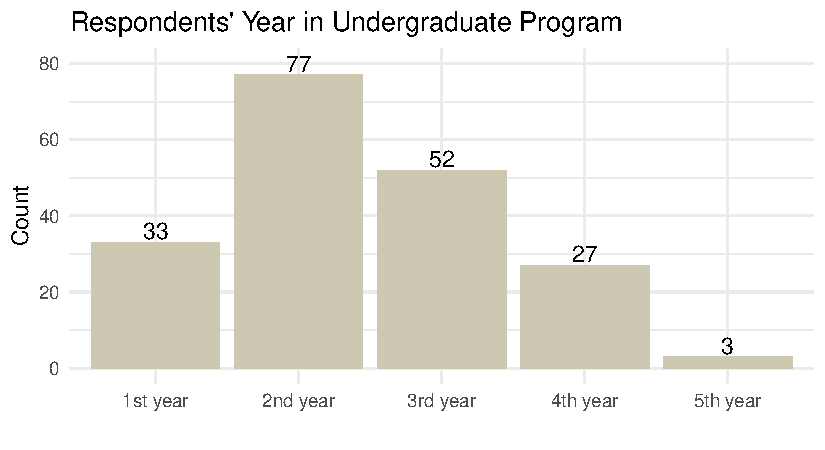
\includegraphics{GlobalHealthQuartoHC_files/figure-pdf/unnamed-chunk-4-1.pdf}

\newpage

As expected, most respondents are between 18-20 years old.

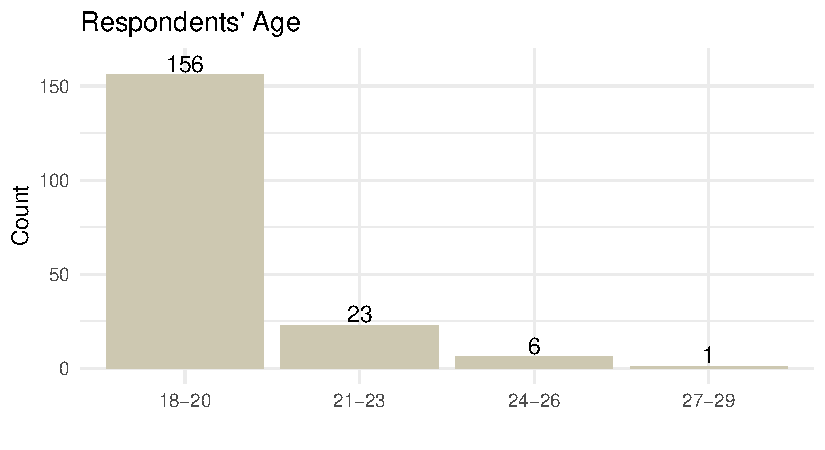
\includegraphics{GlobalHealthQuartoHC_files/figure-pdf/unnamed-chunk-5-1.pdf}

Most of the Respondents are White.

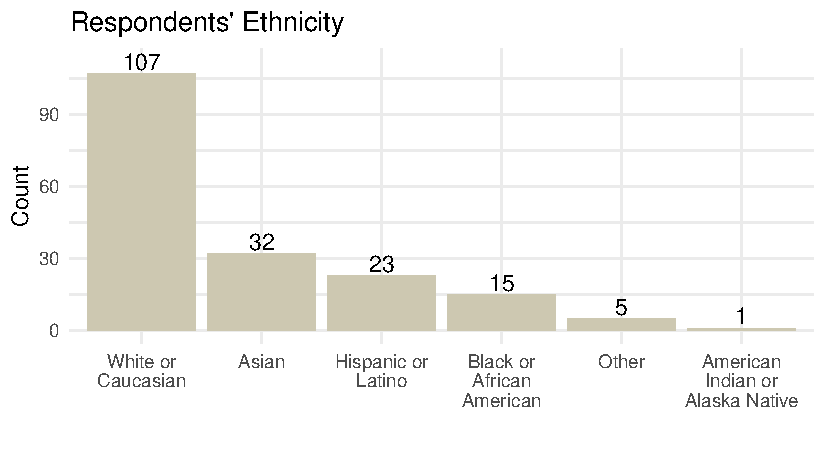
\includegraphics{GlobalHealthQuartoHC_files/figure-pdf/unnamed-chunk-6-1.pdf}

\newpage

A vast majority of the respondents are Women.

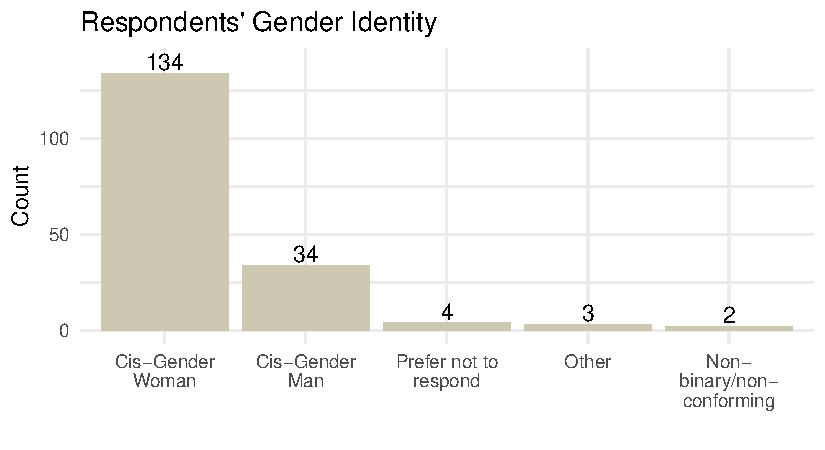
\includegraphics{GlobalHealthQuartoHC_files/figure-pdf/unnamed-chunk-7-1.pdf}

As aforementioned, about half of the respondents attend Baylor
University.

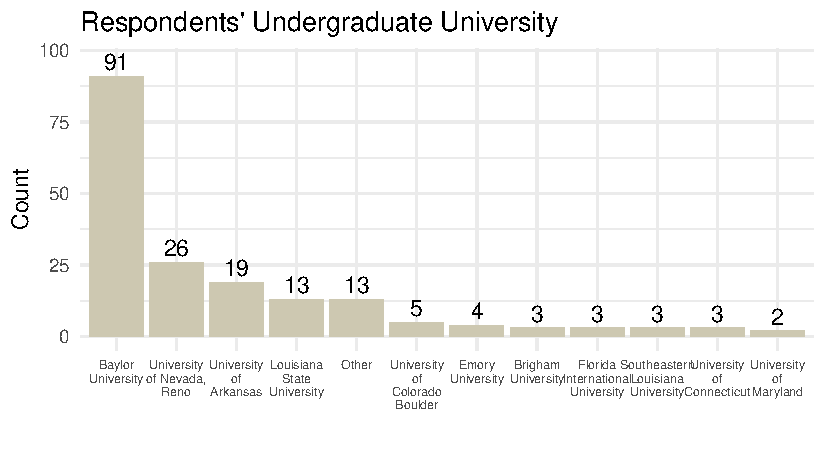
\includegraphics{GlobalHealthQuartoHC_files/figure-pdf/unnamed-chunk-8-1.pdf}

\newpage

Most of the respondents are pursuing the bachelor of science degree.

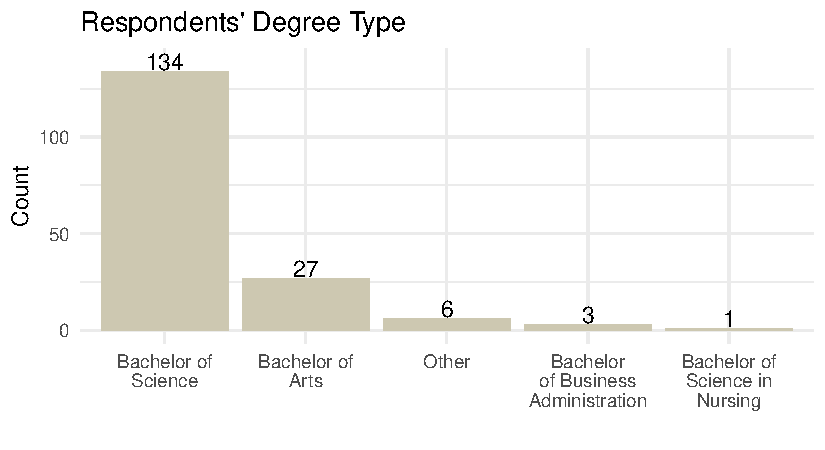
\includegraphics{GlobalHealthQuartoHC_files/figure-pdf/unnamed-chunk-9-1.pdf}

A majority of the respondents' have a natural and physical sciences
major or a public health, health sciences, and nursing major. This is
fitting for a health survey.

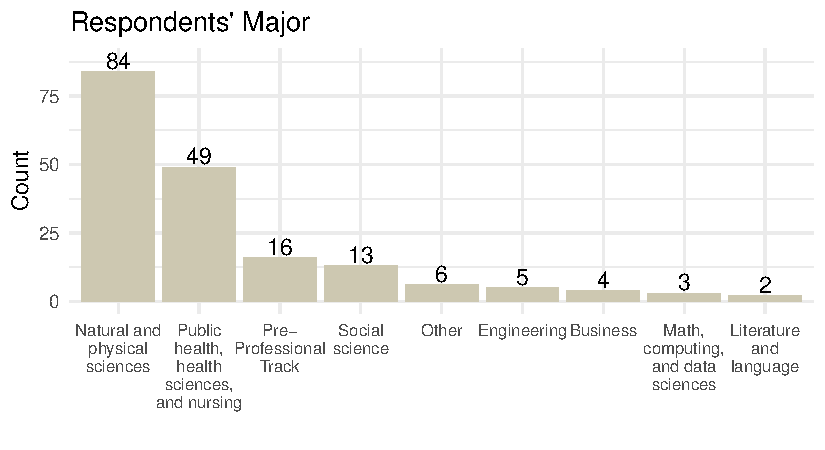
\includegraphics{GlobalHealthQuartoHC_files/figure-pdf/unnamed-chunk-10-1.pdf}

\newpage

The following questions about asking the respondents if they were born
or have lived abroad will be essential for further analysis about Global
Health.

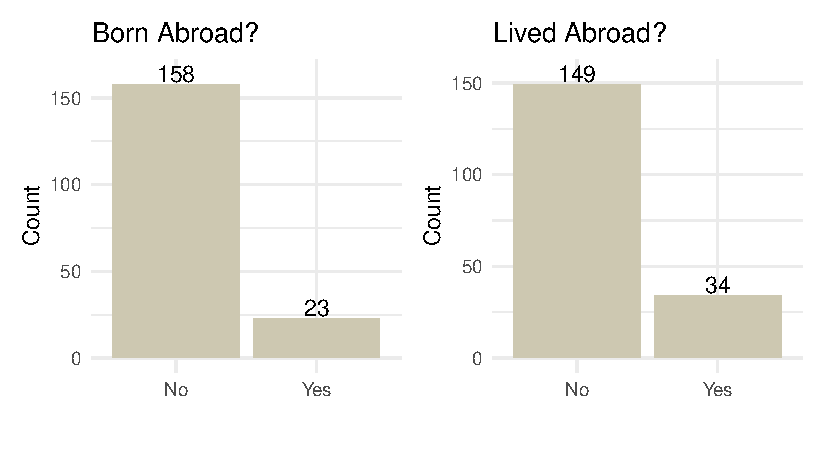
\includegraphics{GlobalHealthQuartoHC_files/figure-pdf/unnamed-chunk-11-1.pdf}

The amount of time that those who did live abroad varies quite a bit. 9
lived abroad for over 15 years, but 9 also lived abroad for 1-5 years.

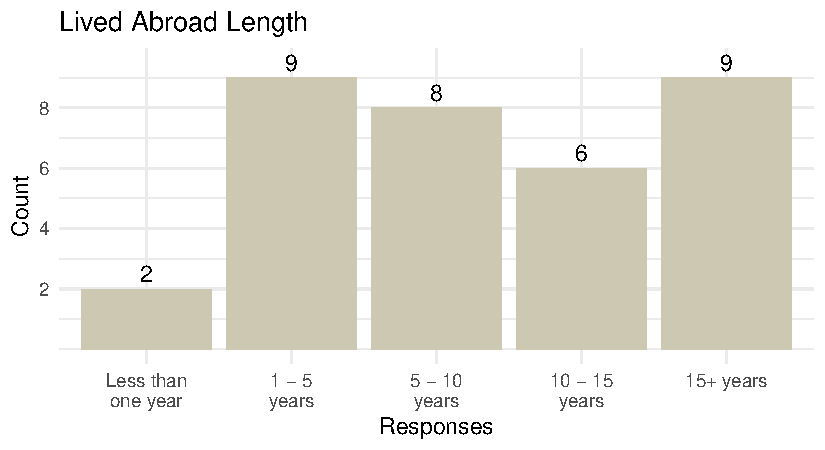
\includegraphics{GlobalHealthQuartoHC_files/figure-pdf/unnamed-chunk-12-1.pdf}

\newpage

\hypertarget{results}{%
\subsection{Results:}\label{results}}

In this section, I will address four of the survey questions that were
most interesting. I will respond to the questions with visualizations
and a few statistical tests to help demonstrate the statistical
significance of the perceived conclusions.

\begin{enumerate}
\def\labelenumi{\arabic{enumi}.}
\tightlist
\item
  How do pre-medical students perceive a career in global health?
\end{enumerate}

Below is a bar graph that demonstrates the overall results to the
question. Most students are interested or uncertain of their interest in
Global Health.

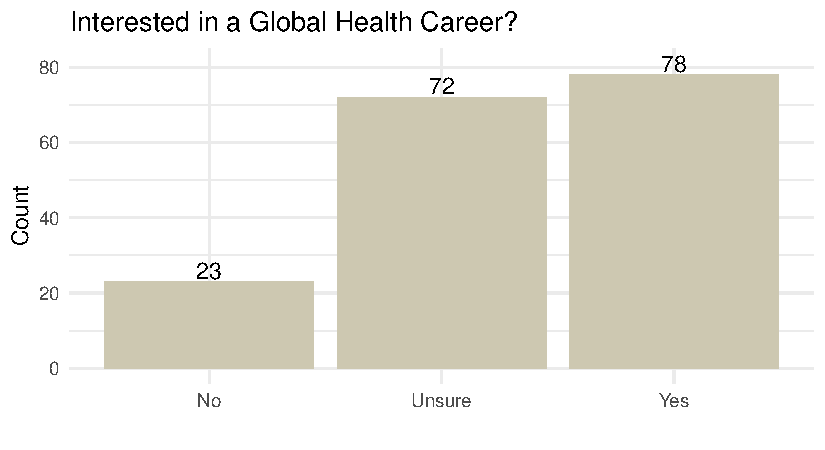
\includegraphics{GlobalHealthQuartoHC_files/figure-pdf/unnamed-chunk-13-1.pdf}

\newpage

1A. Pursuing a career in Global Health grouped by those who have lived
abroad.

Of those who have lived abroad, there seems to be a higher percentage
that want to pursue a career in Global Health. A large portion who have
not lived abroad are uncertain about the idea.

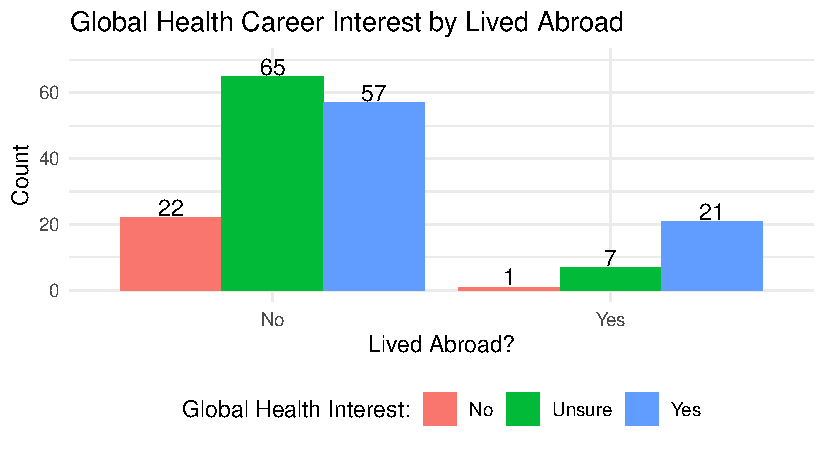
\includegraphics{GlobalHealthQuartoHC_files/figure-pdf/unnamed-chunk-14-1.pdf}

\newpage

The following is a t-test measuring the difference in interest in a
Global Health Career in those who have lived outside the US and those
who have not. For this t-test I counted ``unsure'' responses as 1/2 a
``yes'' and 1/2 a ``no''.

\begin{verbatim}
# 
#   Welch Two Sample t-test
# 
# data:  df14ttest %>% filter(Q12 == "No") %>% select(Q14) and df14ttest %>% filter(Q12 == "Yes") %>% select(Q14)
# t = -3.8394, df = 49.077, p-value = 0.0003537
# alternative hypothesis: true difference in means is not equal to 0
# 95 percent confidence interval:
#  -0.3401720 -0.1064276
# sample estimates:
# mean of x mean of y 
# 0.6215278 0.8448276
\end{verbatim}

The results are significant. Those who have lived outside the US
demonstrate a higher interest in a Global Health Career than those who
have not lived outside the US.

The following is a second t-test measuring the difference in interest in
a Global Health Career in those who have lived outside the US and those
who have not. For this t-test I removed ``unsure'' responses from the
data.

\begin{verbatim}
# 
#   Welch Two Sample t-test
# 
# data:  df14ttest %>% filter(Q12 == "No", Q14 != 0.5) %>% select(Q14) and df14ttest %>% filter(Q12 == "Yes", Q14 != 0.5) %>% select(Q14)
# t = -3.4202, df = 74.733, p-value = 0.001017
# alternative hypothesis: true difference in means is not equal to 0
# 95 percent confidence interval:
#  -0.36876272 -0.09729022
# sample estimates:
# mean of x mean of y 
# 0.7215190 0.9545455
\end{verbatim}

Once again, the results are significant. Those who have lived outside
the US demonstrate a higher interest in a Global Health Career than
those who have not lived outside the US.

\newpage

There does not seem to be an obvious change in responses depending on
the length of time spent abroad.

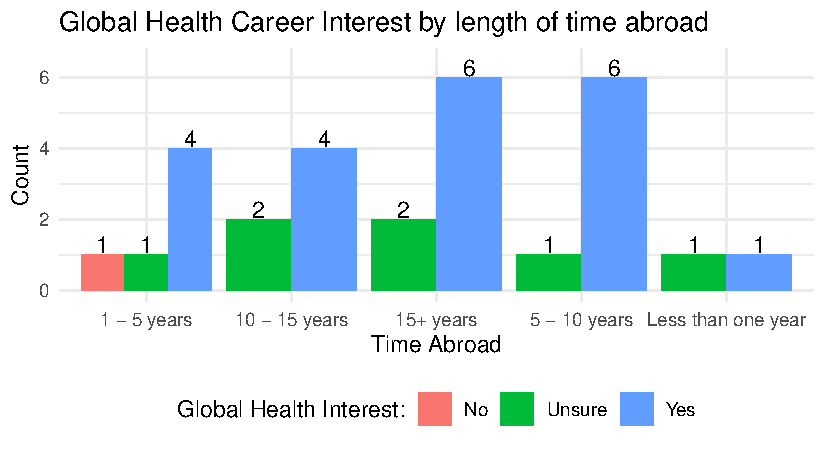
\includegraphics{GlobalHealthQuartoHC_files/figure-pdf/unnamed-chunk-17-1.pdf}

\newpage

1B. Pursuing a career in Global Health grouped by those who were born
abroad.

Again, of those who were born abroad, there seems to be a higher
percentage that want to pursue a career in Global Health. A large
portion who were not born abroad are uncertain about the idea, but a
good about of them are still interested.

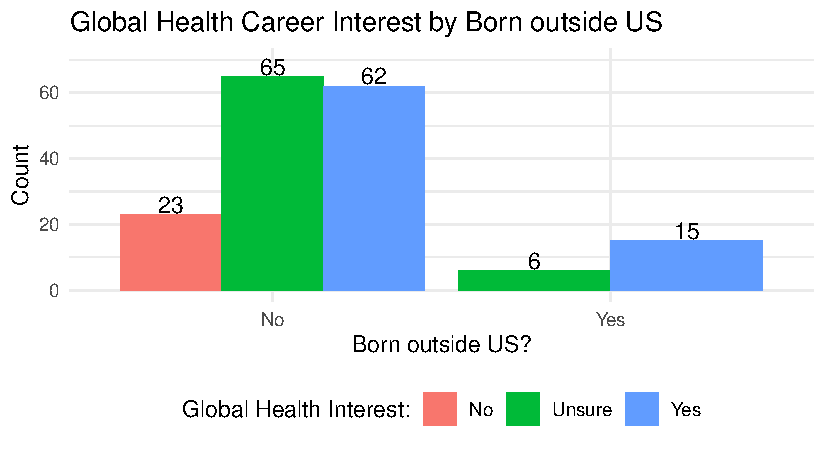
\includegraphics{GlobalHealthQuartoHC_files/figure-pdf/unnamed-chunk-18-1.pdf}

\newpage

The following is a t-test measuring the difference in interest in a
Global Health Career in those who were born outside the US and those who
were not. For this t-test I counted ``unsure'' responses as 1/2 a
``yes'' and 1/2 a ``no''.

\begin{verbatim}
# 
#   Welch Two Sample t-test
# 
# data:  df14ttest %>% filter(Q10 == "No") %>% select(Q14) and df14ttest %>% filter(Q10 == "Yes") %>% select(Q14)
# t = -3.9021, df = 34.782, p-value = 0.000417
# alternative hypothesis: true difference in means is not equal to 0
# 95 percent confidence interval:
#  -0.3453416 -0.1089442
# sample estimates:
# mean of x mean of y 
# 0.6300000 0.8571429
\end{verbatim}

The results are significant. Those who were born outside the US
demonstrate a higher interest in a Global Health Career than those who
were not born outside the US.

The following is a t-test measuring the difference in interest in a
Global Health Career in those who were born outside the US and those who
were not. For this t-test I removed ``unsure'' responses.

\begin{verbatim}
# 
#   Welch Two Sample t-test
# 
# data:  df14ttest %>% filter(Q10 == "No", Q14 != 0.5) %>% select(Q14) and df14ttest %>% filter(Q10 == "Yes", Q14 != 0.5) %>% select(Q14)
# t = -5.5822, df = 84, p-value = 2.848e-07
# alternative hypothesis: true difference in means is not equal to 0
# 95 percent confidence interval:
#  -0.3669824 -0.1741941
# sample estimates:
# mean of x mean of y 
# 0.7294118 1.0000000
\end{verbatim}

The results are significant. Those who were born outside the US
demonstrate a higher interest in a Global Health Career than those who
were not born outside the US.

\newpage

1C. Pursuing a career in Global Health grouped by major.

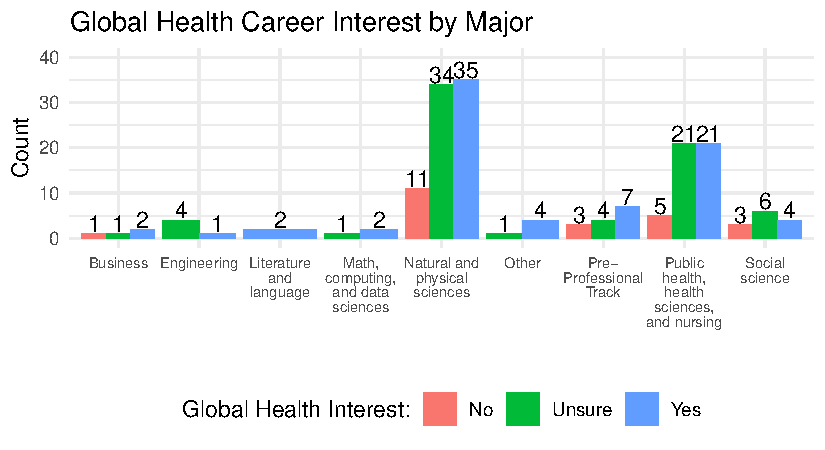
\includegraphics{GlobalHealthQuartoHC_files/figure-pdf/unnamed-chunk-21-1.pdf}

\newpage

\begin{enumerate}
\def\labelenumi{\arabic{enumi}.}
\setcounter{enumi}{1}
\tightlist
\item
  Should all pre-medical students take at least one global
  health-focused class before entering medical school?
\end{enumerate}

Below is a bar graph that demonstrates the overall results. Most
respondents either strongly agreed or agreed that Global Health is a
required course.

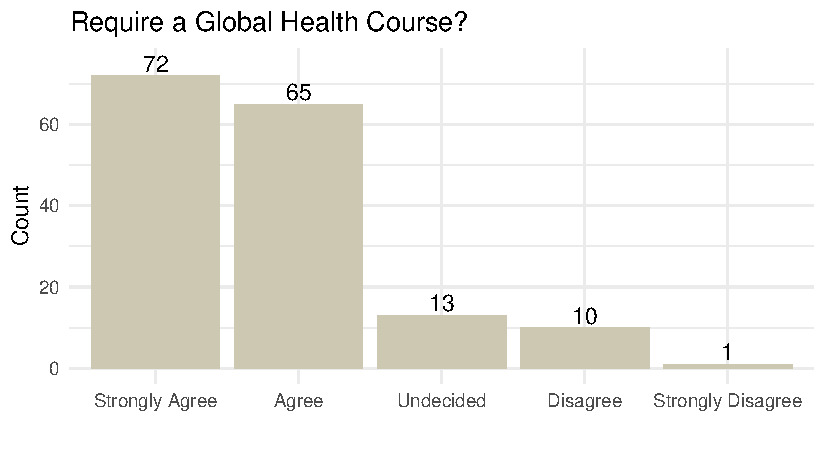
\includegraphics{GlobalHealthQuartoHC_files/figure-pdf/unnamed-chunk-22-1.pdf}

\newpage

2A. Global Health Class Requirement by Global Health Career Interest

It appears that a higher percentage of those interested in Global Health
selected `Strongly Agree' and `Agree' than those who are unsure of their
interest or uninterested.

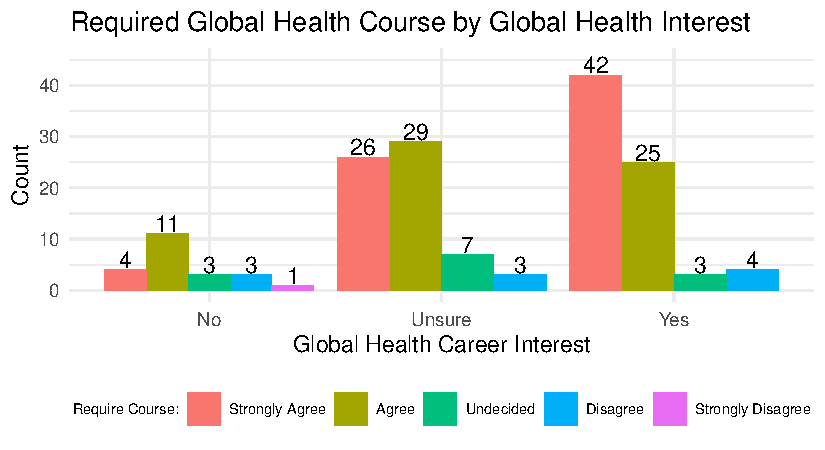
\includegraphics{GlobalHealthQuartoHC_files/figure-pdf/unnamed-chunk-23-1.pdf}

The aforementioned perceptions are made even more clear when the
selections are calculated as percentages. Each Global Health Career
Interest Category totals up to 100\%. This helps to bridge the possible
difference in sample size of the three groups.

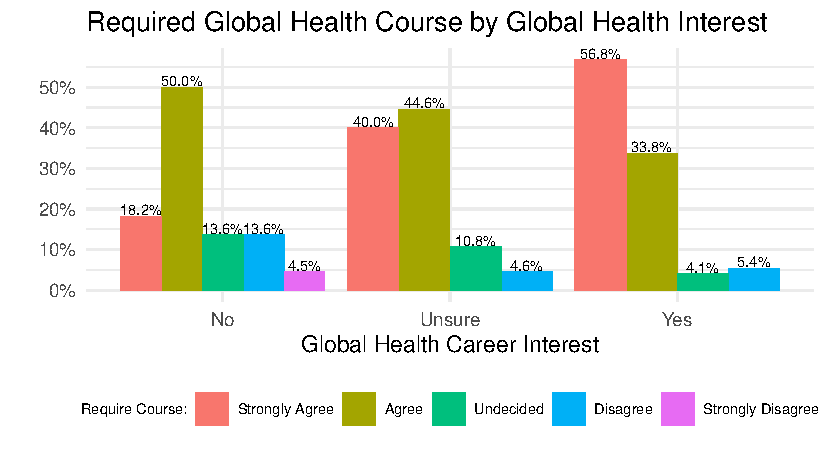
\includegraphics{GlobalHealthQuartoHC_files/figure-pdf/unnamed-chunk-24-1.pdf}

\newpage

2B. Global Health Class Requirement by Living Abroad

At first glance, there is not much distinction between those who have
lived abroad and those who have not lived abroad. Both sections are
dominated by those who agree and strongly agree to the Global Health
Class Requirement.

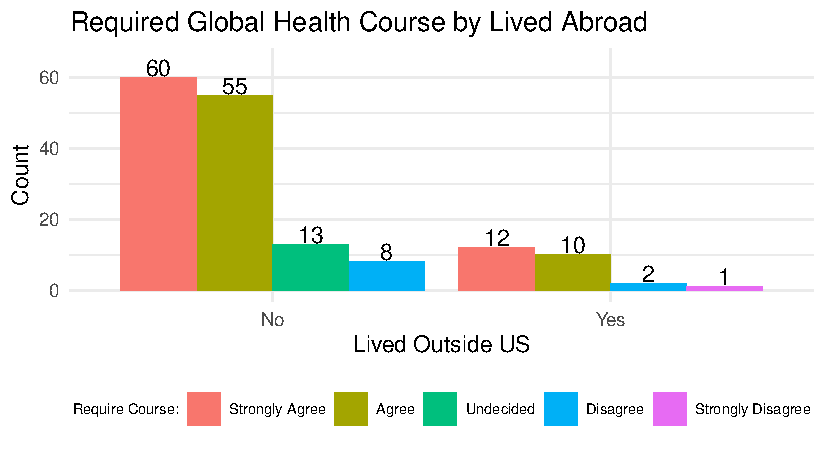
\includegraphics{GlobalHealthQuartoHC_files/figure-pdf/unnamed-chunk-25-1.pdf}

Upon converting the columns into percentages, the similarities are
confirmed. It appears that there is not much difference in those who
lived abroad and those who did not live abroad.

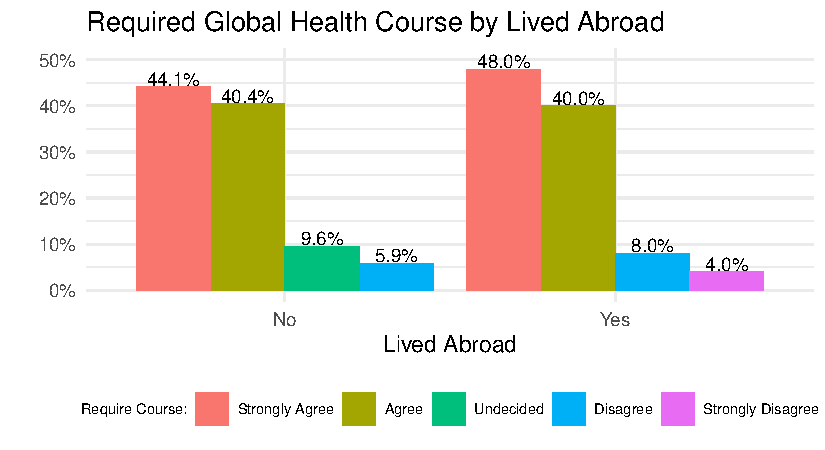
\includegraphics{GlobalHealthQuartoHC_files/figure-pdf/unnamed-chunk-26-1.pdf}

\newpage

2C. Global Health Class Requirement by Major

The below graph differentiates the Global Health Class Requirement by
Major. It is difficult to perceive distinctions because there are so
many natural and physical science, and public health majors.

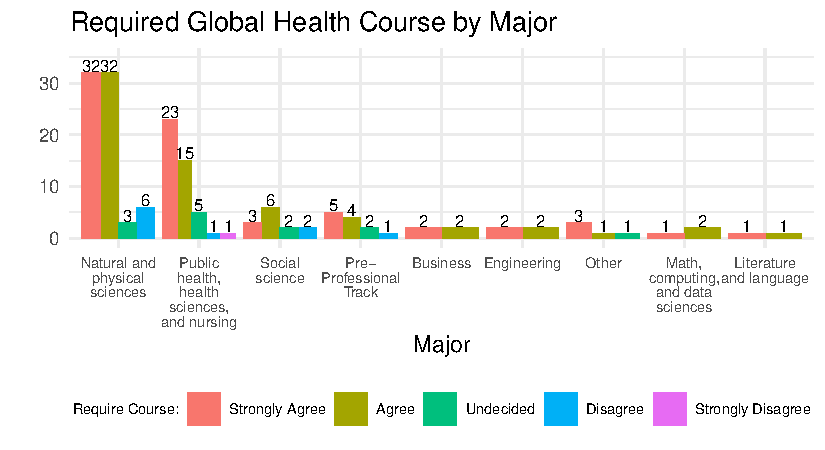
\includegraphics{GlobalHealthQuartoHC_files/figure-pdf/unnamed-chunk-27-1.pdf}

After converting the counts to percentages, it appears that most of the
majors have similar opinions on the Required Global Health Class. It
should be noted, however, that many of these majors have very few
respondents. Realistically, conclusions can only be drawn from the top
two majors: Natural and physical sciences and public health, health
sciences, and nursing.

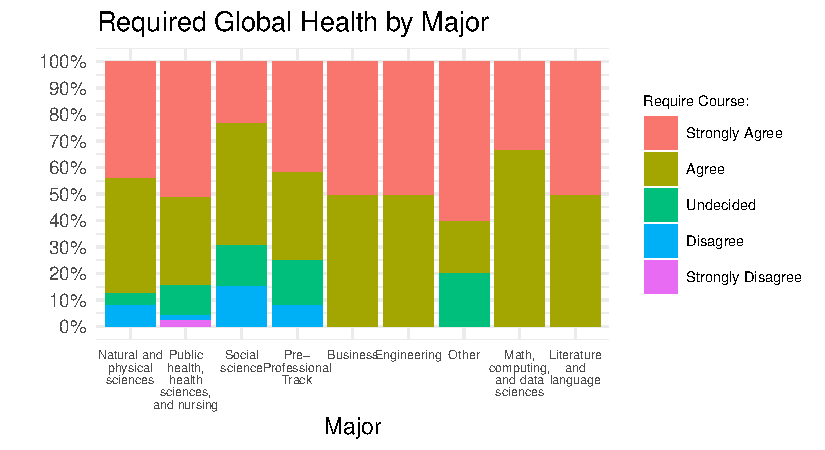
\includegraphics{GlobalHealthQuartoHC_files/figure-pdf/unnamed-chunk-28-1.pdf}

\begin{enumerate}
\def\labelenumi{\arabic{enumi}.}
\setcounter{enumi}{2}
\tightlist
\item
  In your opinion, are there enough global health opportunities
  available to US pre-medical students?
\end{enumerate}

Below is a bar graph that demonstrates the overall results. Most
respondents selected ``I don't know'' or ``No''. Very few chose ``yes''.

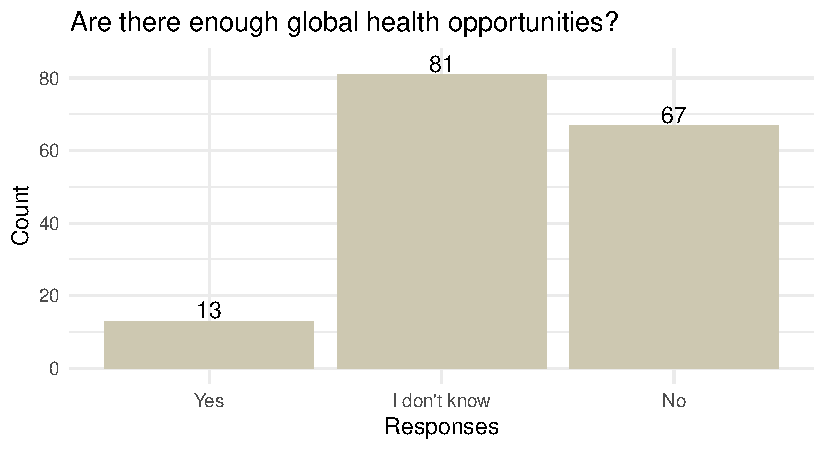
\includegraphics{GlobalHealthQuartoHC_files/figure-pdf/unnamed-chunk-29-1.pdf}

\newpage

3A. Global Health Opportunities by Global Health Career Interest

It appears that those that are interested in a career in Global Health
are much more likely to answer that there are not sufficient Global
Health Opportunities. Most of those that are uninterested or unsure of
their interest in Global Health are unsure of the extent of Global
Health opportunities.

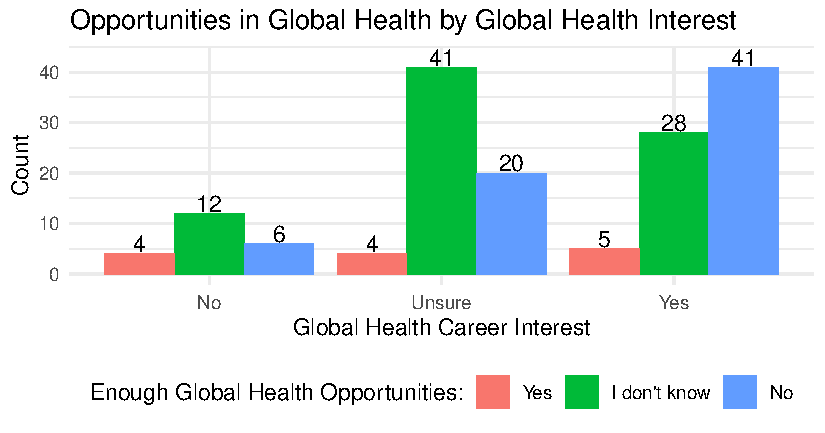
\includegraphics{GlobalHealthQuartoHC_files/figure-pdf/unnamed-chunk-30-1.pdf}

After converting the counts into percentages, it is evident that a large
portion of those uninterested and uncertan of their interest in Global
Health are unsure if there are enough Global Health Opportunities.
Almost double the proportion of those who are interested in a Global
Health career think there are not enough Global Health Opportunities.

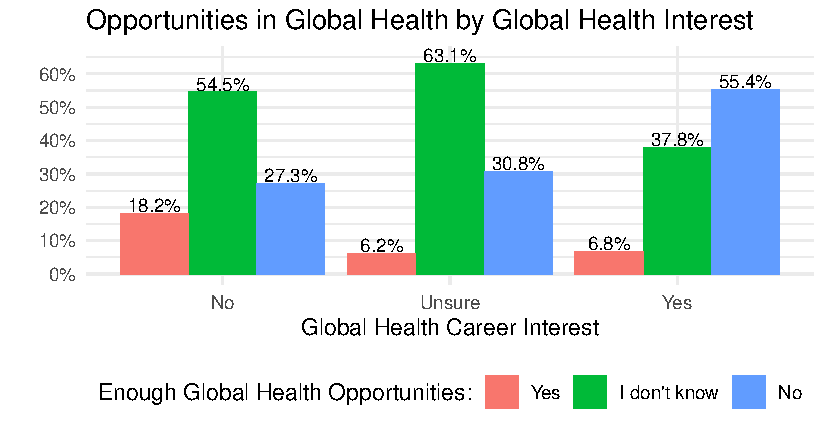
\includegraphics{GlobalHealthQuartoHC_files/figure-pdf/unnamed-chunk-31-1.pdf}

\newpage

The following is a t-test measuring the difference in belief that there
are sufficient Global Health opportunities for pre-med students in those
who have expressed interest in a Global Health Career and those who have
not. For this t-test, I counted ``I don't know'' responses to the
sufficient Global Health Opportunities Question as 1/2 a ``yes'' and 1/2
a ``no''.

\begin{verbatim}
# 
#   Welch Two Sample t-test
# 
# data:  df18ttest %>% filter(Q14 == "No") %>% select(Q18) and df18ttest %>% filter(Q14 == "Yes") %>% select(Q18)
# t = 2.4289, df = 32.145, p-value = 0.02091
# alternative hypothesis: true difference in means is not equal to 0
# 95 percent confidence interval:
#  0.03194622 0.36363118
# sample estimates:
# mean of x mean of y 
# 0.4545455 0.2567568
\end{verbatim}

The results are significant. Those who have express an interest in a
Global Health Career indicate that there are not sufficient Global
Health Opportunities at a higher rate than those who have not expressed
an interest in a Global Health Career.

The following is a second t-test measuring the difference in belief that
there are sufficient Global Health opportunities for pre-med students in
those who have expressed interest in a Global Health Career and those
who have not. For this t-test, I removed all ``I don't know'' responses.

\begin{verbatim}
# 
#   Welch Two Sample t-test
# 
# data:  df18ttest %>% filter(Q14 == "No", Q18 != 0.5) %>% select(Q18) and df18ttest %>% filter(Q14 == "Yes", Q18 != 0.5) %>% select(Q18)
# t = 1.7159, df = 10.498, p-value = 0.1155
# alternative hypothesis: true difference in means is not equal to 0
# 95 percent confidence interval:
#  -0.08453279  0.66714149
# sample estimates:
# mean of x mean of y 
# 0.4000000 0.1086957
\end{verbatim}

The results are not significant. This is likely because a large amount
of respondents selected ``I don't know.'' This drops the sample size to
only 80.

\newpage

\begin{enumerate}
\def\labelenumi{\arabic{enumi}.}
\setcounter{enumi}{3}
\tightlist
\item
  Which, if any, of the following do you perceive as reasons it is
  difficult for undergraduate pre-medical students to learn more about
  global health and gain experience in the field prior to medical
  school?
\end{enumerate}

Below shows the immediate results to the question. It seems Busyness and
Finances are the two largest hindrances to Global Health Awareness and
Access. The plot includes the counts of each response as well as the
percent of the respondents that selected each hindrance. A notable
83.4\% of respondents indicated that busyness is a large hindrance to
Global Health Awareness and Access.

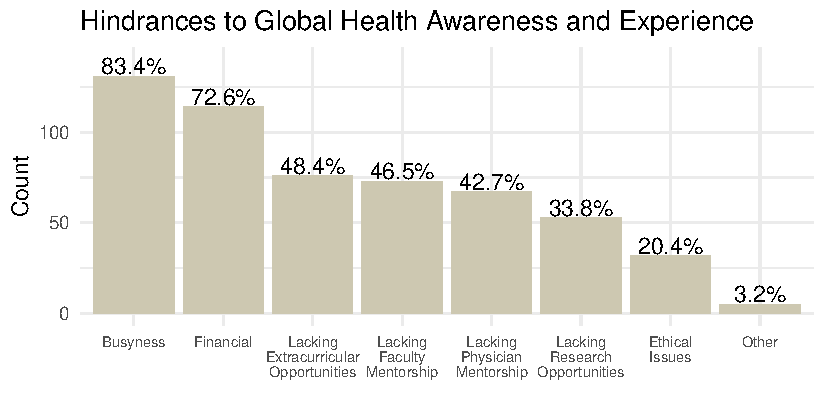
\includegraphics{GlobalHealthQuartoHC_files/figure-pdf/unnamed-chunk-34-1.pdf}

The question allowed the respondents to select multiple hindrances. This
graph shows the total number of hindrances that each respondent
selected. Most respondents chose between two and four.

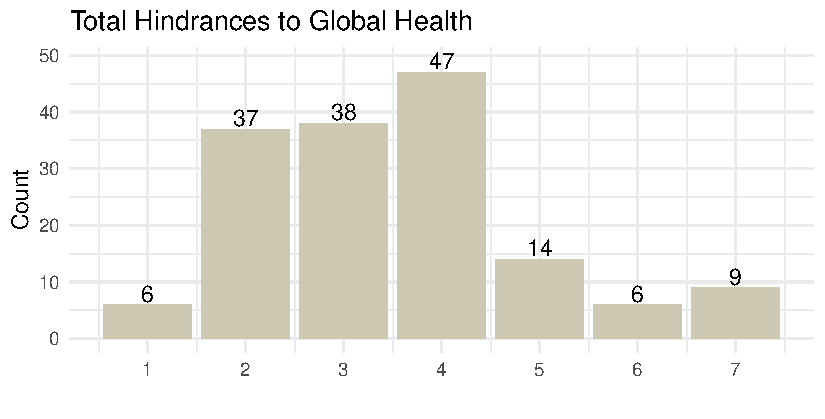
\includegraphics{GlobalHealthQuartoHC_files/figure-pdf/unnamed-chunk-35-1.pdf}

\newpage

\hypertarget{conclusion}{%
\subsection{Conclusion:}\label{conclusion}}

There are a few general conclusions that we can draw from the surveys.
First, a sizable amount of undergraduate students are interested in a
career in Global Health. There are also a large amount that are
uncertain about their interest. Living and being born abroad have a
significant correlation with this interest.

A large amount of those interested in a career in Global Health are
convinced that there are not enough opportunities to gain awareness or
experience in Global Health.

One possible response to this is requiring a Global Health Course to
enter medical school. A sizable majority of students agreed that this
was a good idea. As expected, this majority increased drastically if a
student was already interested in Global Health.

The respondents have identified a few different hindrances to a Global
Health Career. The most commonly selected were busyness and finances.

Altogether, it is difficult to draw significant conclusions from a
survey like this. The sampling is not perfect, and far from
comprehensive of the entire United States. There are not enough
respondents and some of the questions are broad and open ended. Still,
it gives the readers a good idea of undergraduates' general perception
of Global Health. Hopefully this will open up future, more comprehensive
surveys to come.

There are several more questions that I have analyzed that were not
selected in this Honors Contract Report. These could provide further
illumination on the subject.



\end{document}
